% Comments --
% 12/10/12 -
%  - incorporate previous work on CRDTs by Preguica, Weiss,  Urso, Molli, Oster, etc.
%
% 03/01/10 - 
%   -Benchmark space complexity of Node extension vs node of size one
%   -Explain the three types of linked lists (section 6)
%   -Work the clash example with the hashtable for node ids, linked list of
%    of global subnodes, linked list of local subnodes.
%   -Create git repository for Dissertation and Collabed.
%   -
% 02/23/10 - Work on the optimization section and lead it into experimental
% results.

% Future work: Intention preserving; Why our approach could really preserve
% a cut and paste (via tree-node transplant) and OPT can't

% 02/17/10 - Starting a new collabed session of the MSET paper.
%     This paper, along with all the images and scripts are
%     stored in a git repository on pythia as "paper-collabed.tex"
%     at address "pythia.cs-i.brandeis.edu/git/mset_paper"

% 7/28 - completed first draft of the paper through the algorithm
%     we still need to add more figures and to revise to make it
%     more readable



\documentclass{amsart}

\usepackage{epsfig}
\usepackage{graphicx}
\usepackage[all]{xy}
\usepackage{pb-diagram}
\usepackage{ulem}

\newtheorem{theorem}{Theorem}[section]
\newtheorem{lemma}[theorem]{Lemma}
\newtheorem{proposition}[theorem]{Proposition}
\newtheorem{corollary}[theorem]{Corollary}



\title{Optimally Efficient Collaborative Text Editing}
%
%


\author{
Kenroy~ G.~ Granville
\and 
Timothy J.~Hickey 
}
%\authorrunning{Hickey  and Granville}
%\tocauthor{Timothy J.~Hickey (Brandeis University)
%\and Kenroy~ G.~ Granville (Brandeis University) }
%\institute{Computer Science Department, Brandeis University \\
%\email{\{tim$\mid$kgg\}@cs.brandeis.edu} }

\bibliographystyle{abbrv}

\begin{document}

\maketitle

\begin{abstract}
In this paper we present a new collaborative text editing data type,  
the Monotone Shared Edit Tree (MSET). This algorithm is an extension
and optimization of the TreeDoc datatype of Preguica and Shapiro.  The MSET data type is an example of
a Commutative Replicated Data Type. It is not based on operational transformation 
and does not require a central server to serialize the
edit operations.
MSET allows multiple users to locally 
edit their own copies of a shared text document
while simultaneously sending out their local edits 
to remote users and processing edits from remote users 
on their local copy.
Each edit operation (whether generated locally or remotely) 
requires $O(k\log(M))$ time to process, where
M is the total number of characters that have inserted 
into the user's document before the operation in
question is applied (including those characters that were later deleted.)
The MSET algorithm is based on 
the Model-View-Controller paradigm in which the
model underlying the text document is a simple and 
natural type of tree that represents the full collaborative edit process.
The edits that are allowed for this tree are monotone in the sense that
the individual edits add a component to the tree which can never be removed
though it can be evolved. For example, deletion is handled by setting the
visibility attribute of the character to ``hidden''. The operations are also
designed to facilitate shared editing in the sense that the order in which
they are applied does not affect the eventual result.
The MSET algorithm is convergent in the sense that 
if all users stop generating
editing operations, then when all operations have 
been received and processed, all users will have
the same document. 
A collaborative editor based on the MSET algorithm 
has been successfully introduced as a plugin into widely used
editors such as JEdit and Netbeans and 
these collaborative editors have been used in classroom situations
with positive feedback from the users (both students and faculty).
\end{abstract}
\newpage
\tableofcontents
\newpage

\section{Introduction}
Collaborative text editing has a long history stretching back to the dOPT model of Ellis and Gibbs from 1989 \cite{ellis_concurrency_1989}. Most of the early work on collaborative editing used an operational transformation approach with a central server that would serialize all edit operations and rebroadcast them to the clients \cite{nichols_high-latency_1995}. The server and clients would transform the edit operations before applying them to account for differences in the remote documents when the original edit operations were applied. Many extensions and variations of this early work have been developed over the ensuing 25 years (see e.g. \cite{sum_operational_2004}).

In the past few years, a new approach has been developed that greatly simplifies the process of collaborative editing by relying on data types in which the edit operations are commutative and hence do not need to be transformed. These include Uniwiki \cite{oster_building_2010, oster_uniwiki_2009},  TreeDoc \cite{ letia_consistency_2010, preguica_commutative_2009}, WOOT \cite{oster_data_2006}, LOGOOT \cite{weiss_logoot:_2008, weiss_logoot:_2009, weiss_logoot-undo:_2010}, WOOKI \cite{weiss_wooki:_2007}. 

Our work, MSET, is a generalization and optimization of the TreeDoc data type  of Preguica, et. al.  \cite{preguica_commutative_2009}. It has been available since 2007 as an open source project hosted at sourceforge (http://collabed.svn.sourceforge.net/viewvc/collabed/src/) and has been used as the foundation of the CollabEd system  \cite{granville_collabed:_2009}, which provides a common plugin architecture for code editors allowing developers on different platforms (e.g. jEdit, NetBeans, Eclipse) to collaboratively edit a code file while still using the IDE that they prefer.

In the rest of this paper we give an overview of the central problems faced by collaborative editors and then we introduce the MSET data type.  The first version is an unoptimized data type which is a simple extension of the TreeDoc model. We then show how to optimize the operations so that every insert or delete operation has time complexity $O(k\log(M))$ for the client originally performing the operation and for each client that receives the broadcasted operation. In contrast to the approach used in TreeDoc, we do not need to rebalance the tree to obtain optimal performance.



\subsection{The Collision Problem}
The fundamental problem in collaborative editing of any documents  
(of any type, not just text)
is dealing with collisions that occur when two 
users (say $A$ and $B$) apply different operators (say $\alpha$ and $\beta$) 
to a shared document. Assuming that both users
start off with the same document $D$, the two users will have two (usually) 
different documents $\alpha(D)$ and $\beta(D)$.
A collaborative editor needs to resolve this conflict, so that both users 
return to the state of having the same document $D'$.
This can be done 
by introducing transformed operations $\alpha'=T_\beta(\alpha)$ and 
$\beta'=T_\alpha(\beta)$ as shown in the diagram below,
where $T$ is a transform operator:
\[
\begin{diagram}
\node{D} \arrow{e,t}{\alpha} \arrow{s,l}{\beta} \node{\alpha(D)} \arrow{s,r}{\beta'=T_\alpha(\beta)} \\
\node{\beta(D)} \arrow{e,t}{\alpha'=T_\beta(\alpha)} \node{D'}
\end{diagram}
\]
and the transform operator must be defined so that this diagram commutes, 
that is, there must be an operator $\gamma$ on
$D$ such that:
\[
\alpha'(\beta(D)) = \beta'(\alpha(D)) = \gamma(D)
\]
If this operation holds, we can let $(\alpha \vert \beta)$ denote the combined operation $\gamma$.

If the operators are invertible then one can define 
the transform operator $T$ in terms of the collision
operator $\gamma$, as follows. Since the operators $\alpha$ 
and $\beta$ are invertible, there must be
operators $\alpha^{-1}$ and $\beta^{-1}$ such that
\[
\alpha^{-1}(\alpha(D)) = D \;\;
\beta^{-1}(\beta(D)) = D 
\]
we then define T as follows:
\[
T_\alpha(\beta) = (\alpha \vert \beta) \circ \alpha^{-1}
\]
Once a collision operator is defined, 
one can implement a collaborative editor which uses a central
server to serialize all of the edit operations into a single stream 
and which applies the transforms to resolve
conflicts among users.  We provide an overview of such a server in the appendix.
% TODO: include a citation here

There are some problems with collaborative editors implemented
using the the Operational Transformation model.  One problem is that the
collision operators need to be implemented in a way that is natural and
intuitive for the users.  Another is that if the latency is high, the time
required to transform individual operations can be unacceptably large. In
bad cases, the time to process a remote edit operation can be quadratic
in the size of the edit-string. We present this analysis in the appendix.
% TODO: check to see if this is needed ...

In this paper we present a new algorithm based on a more sophisticated
representation of the string. We call this the 
{\bf Monotone Shared Edit Tree} or MSET representation. 

In the next section we provide an overview of the new MSET-based
collaborative editing algorithm.
Then we introduce a sequence of collaborative editors of increasing sophistication
starting with a collaborative tree editing algorithm and moving down to a collaborative
string editing algorithm which transforms string operations into tree operations.
After describing the fundamental algorithms we present an optimally efficient
implementation which requires $O(N\log(N))$ time for $U$ users to perform
a collaborative edit of a document consisting of $N$ insertions and deletions of
single characters, more precisely $N$ is the sum of the sizes of all strings that
were inserted or deleted by any user from the document. This does not include the
time for broadcasting the messages over the network. Each individual operation
requires time $O(k*\log(N))$ where $k$ is the number of elements inserted or deleted
and $N$ is the total number of elements that have been inserted or deleted so far.


\section{Overview of the MSET algorithm}

In this paper we propose a method for collaborative editing in which the
users maintain a tree-structured representation of the editing process and
broadcast tree edit operations rather than string-edit operations. The advantage
of this approach is that the tree-edit operations we introduce do not need to be transformed
(that is they commute -- $\alpha(\beta(T)) = \beta(\alpha(T))$) This greatly increases
the efficiency of the collaborative editing scheme. 


There are several key features of the MSET model:

\paragraph{\bf simple model}
The underlying tree model is a simple and natural tree representation
of the collaborative edit session.

\paragraph{\bf local}
All users transform the string operation into a tree operation
which is performed locally.

\paragraph{\bf peer-to-peer}
The tree operations, once performed locally, are broadcast
to all other users, either using a central server or a peer-to-peer approach.
Users receive remote tree operations (in any order) though some must
be cached if their target node has not yet been created locally.

\paragraph{\bf convergent} 
When all users stop editing and all messages are delivered and processed, all
users will have the same edit-tree and hence the same standard and edit-string
views.

\paragraph{\bf optimally efficient}
Each operation takes time $O(k\log(M))$ where $k$ is the number of characters
inserted or deleted and $M$ is the size of the edit-string.

\paragraph{\bf generalizable}
The model can be easily generalized so that each character can have attributes
from any attribute set (font, style, color, etc.) and any user can change the
attributes at any time. Visibility can be one of those attributes, so that 
characters can be hidden and unhidden at any time. The properties above 
all remain for this more general model, except that the model is slightly
more complex.

\paragraph{\bf practical} 
This model has been used to create colloration plugins for several
popular editors and IDEs including JEdit and NetBeans. These
collaboratized editors have been used in Computer Science classes
and have been found easy and natural to use by students and faculty
alike.

\subsection{Comparion to Operational Transformation}
The collaborative editing algorithms based on Operational Transformation generally satisfy the three properties listed below.
As we explain, MSET satisfies the first, doesn't satisfy the second, and may or may not satisfy the third depending on whether
cut/paste operations are allowed as atomic operations.
\begin{enumerate}
\item {\bf convergence property} - after all editing has ceased and the system has become quiescent then all users will
have exactly the same document.  We will prove that the MSET algorithm is convergent. 
\item {\bf causality preservation} - if a given user performs operation A before operation B, then for all other users
the transformed operation A is performed before the transform of the operation B.  The MSET algorithm 
{\it is not causality preserving}. 
For example, if a user inserts several
substrings into an initial string $\alpha$, then the algorithm will not necessarily preserve the order in which those operations
were performed when they are sent to the other members of the collaborative editing group.
\item {\bf intention preservation} - if a given user performed an operation A on a document, then the transform of that operation
should have the same ``intention'' when it is performed in all other user's documents. 
The MSET algorithm is intention preserving in an editing regime that only allows insertion and
deletion, but it is not intention preserving if one also allows cut/paste as an atomic operation. More precisely, if user A is working
on a section of a document and user B cuts away a substring containing A's work and then paste's that section into another part
of the document. One might expect that A's position in the string would be moved to the new part of the string and although 
A might find this transport disorienting, at least there would be no break in the continuity of ``A's'' editing.  
This is not what happens with MSET.
Indeed, User A would suddenly find the text around his/her position deleted and, if there was some latency, 
the characters A had been typing would appear in this deleted region. User A will then have to search for the moved text.
\end{enumerate}


\subsection{A simple example of the MSET algorithm}
Let us assume that we have several users $u_0,u_1,\ldots$ who are
collaboratively editing a shared document. Each user maintains a local
copy $\alpha_i$ of the string being edited and also maintains a more complex representation of the editing process
which we will call an edit-tree.
This edit-tree $T_i$ represents the string and all edits that have been
performed on it. There is a natural projection $f$ from edit-trees to
strings such that $f(T_i)=\alpha_i$ and this invariant will be maintained.
The users can also switch to a "edit-string" view 
$g(T_i)=\beta_i$ of the document
which shows a string-representation of the tree. The examples below will
make this clear.

\subsubsection{Initial state}
All users start out with the empty string $\alpha_i=""$ where the
tree representation $T_i$ is a single node owned by user $u_0$, the superuser,
and containing only the start and end marker symbols $<^0_0$ and $>^0_0$
which only appear in the edit-string view.
\[
g(T_i) \;=\; <_0^0 \;\;\;\;\;\; >_0^0
\]
Although the users can insert anywhere in the standard view of their document,
they can only insert in certain locations in the edit-string view.
For example, in this initial edit-string, 
the users can only insert between the two markup nodes.

Each node in the edit-tree is owned by
a single user $u$ and the nodes owned by a user $u$ also have an index $n$
which uniquely identifies them for that user. Thus each node
is uniquely identified by the pair $u/n$ of user id and node index.
The index $n$ is the number of nodes that have been created by $u$ before
the current node so it doesn't depend on how many nodes any other user
has created. It is a purely local counter for user $u$.

The user $u_0$ represents the
system and owns only one node, the root. User $u_0$ also does no editing on
the document.

\subsubsection{Inserting a string}

If user 1 then inserts the sentence ``This is an example.'' 
the string operation on $\alpha_1$ is
\begin{verbatim}
  insert(0,"This is an example")
\end{verbatim}
which is translated into the following edit-tree operation
\begin{verbatim}
  insert(u0/n0,0,u1/n0,"This is an example")
\end{verbatim}
which states that a new node, $u1/n0$, should be inserted as a child of
node $u0/n0$ at position $p=0$. This operation is then broadcast to all of the
peers who apply it to their own trees $T_j$.
The corresponding edit-tree is shown in Figure \ref{fig:tree0} and the
corresponding edit-string is
the edit-string $\beta_1$ becomes
\[
<_0^0 <_0^1 \text{This  is  an  example.}>_0^1 >_0^0
\]
In practice, user 1 would insert the sentence one character at a time
and the node would be constructed incrementally.
After inserting the first character ``T'' the node $(u1/n0:1)$ would be created
containing only the letter ``T''. After inserting the next character, ``h'',
the system would generate an {\tt extend} operation which would add the
next letter to the end of the node. This is only possibly if the user making
the extension is the owner of the node and if the new character is inserted
at the end of the node.



\begin{figure}[h]
\centering
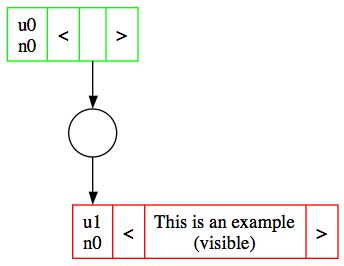
\includegraphics[width=2.0in]{tree1zz.jpg}
\caption{Tree after inserting "This is an example.\label{fig:tree0}"}
\end{figure}

\subsubsection{Inserting a substring}
Next suppose that the user 1 decided to insert the word "interesting"
before "example."  This can not be handled as an extension of the node
$u1/n0$.  As above, this will actually be inserted one character at a time
in most cases (unless the user cut and pastes the word from some other
document into the buffer). Since this is an insertion in the middle of a node,
the system will generate a tree-edit operation which adds a new node $u1/n1$
containing the character $i$ and attaches that node at position 11 of the
parent node $u1/n0$.  As the user continues to type the word "interesting"
the successive characters are added to the node $u1/n1$ as $u1$ is the owner
of the node and the insertions are at the end of the node. The result
is a new node containing the entire word "interesting" attached at position
11 of its parent. The tree in the left side of Figure \ref{fig:tree11}
shows the resulting edit-tree.



\subsection{Creating conflicts in collaborative editing}
Next, suppose user $u3$ 
simultaneously inserts the adjective "illustrative "
before the word "example" in their own
local copies and that both users broadcast their edits to their peers, which
includes user 2 who is just watching the other two edit.  
In a high latency environment (or in a setting where the user's are queueing 
their edits before sending them out), user 2 would create its own tree
but with a different node attached at position 11 of the $u1/n0$. This tree
is shown in the right side of Figure \ref{fig:tree11}. Again, if user 3
is typing the word character by character then the first character will generate
the node $u3/n0$ containing only one character.

Lets look at this more closely.
We assume at a given point in time all users share the same edit-tree as shown 
in Figure \ref{fig:tree0}. Then they all have the string view
\[
\alpha_i= \text{"This is an example."}
\]
Now, if user 1 applies the string operation
\begin{verbatim}
  insert(11,"interesting ")
\end{verbatim}
this will be translated into the following edit-tree operation
\begin{verbatim}
  treeinsert(u1/n0:19,11,u1/n1,"interesting ")
\end{verbatim}
which states that the new node $u1/n1$ containing the text "interesting"
should be added as a child of the node $u1/n0$ at position 11 out of 19. Applying
this operation results in the edit-tree in the left side of Figure \ref{fig:tree11}
and in the following edit-string view
\[
 <_0^0 <^1_0 
 \text{This is an }<^1_1 
 \text{interesting}
>^1_1  \text{example.} >^1_0 >_0^0
\]
Similarly for user 3 who applies the string operation
\begin{verbatim}
  insert(11,"illustrative ")
\end{verbatim}
which is translated into the following edit-tree operation
\begin{verbatim}
  treeinsert(u1/n0:19,11,u3/n0,"illustrative ")
\end{verbatim}
resulting in the following edit-string corresponding to the edit-tree
in the right side of Fig \ref{fig:tree11}
\[
 <_0^0 <_0^1 
 \text{This is an} <^3_0 
 \text{illustrative}
>^3_0  \text{example.} >_0^1 >_0^0
\]


\begin{figure}[h]
\vspace{\baselineskip}
  \hspace{\fill}\rule{\linewidth}{.7pt}\hspace{\fill}
  \vspace{\baselineskip}

\centering
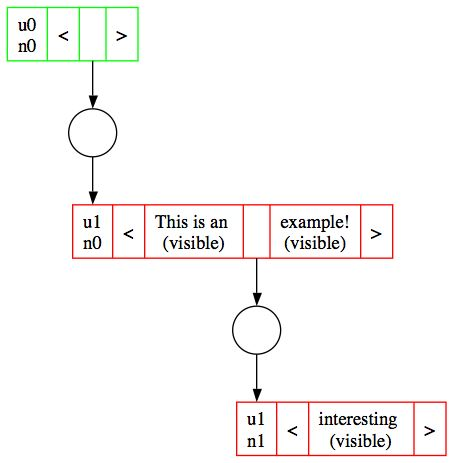
\includegraphics[width=2in]{tree11.jpg}
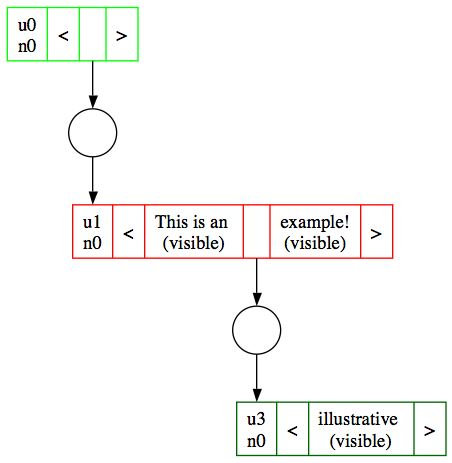
\includegraphics[width=2in]{tree12.jpg}
\caption{Tree $T_1$ on the left after user 1 inserts "interesting ,
and tree $T_3$ on the right after user 3 inserts "illustrative ".\label{fig:tree11}}

\centering
\vskip 0.3in
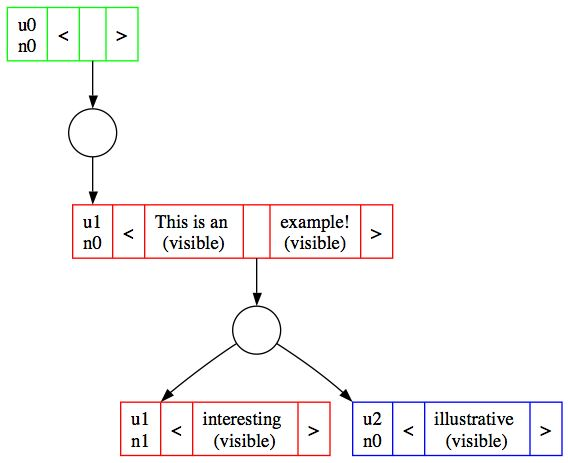
\includegraphics[width=3in]{tree13.jpg}
\caption{Trees after inserting both "interesting " and "illustrative ".\label{fig:tree13}}


\vspace{\baselineskip}%
  \hspace{\fill}\rule{\linewidth}{.7pt}\hspace{\fill}%
\vspace{\baselineskip}%
\end{figure}

\subsection{Handling conflicts in collaborative editing}
When user $u_2$ receives these tree-edit operations there will be an
apparent conflict. Both $u1$ and $u2$ want to insert a string at position
$11$ of $u1/n0$.  

The MSET approach is to allow multiple users to insert at
the same position, but to order the insertions by user id, and to disallow
the same user from inserting multiple times at the same position in the edit-tree.
Thus, if there are $k$ users, then there could be up to $k$ children nodes
attached at any particular position of an edit-tree node.

In this case, conflict resolution results in the tree in Figure
\ref{fig:tree13} where $u1/n0$ has two children nodes attached at position $11$,
the node $u1/n1$ is on the left and $u3/n0$ on the right as $u1<u3$.
This strategy for handling conflicts guarantees that all users will have
the same edit tree, no matter which order they apply the edit-tree operations.

In the case where the new nodes were created one character at a time, rather
than using cut/paste to insert the words, the conflict would occur with two
nodes that each contain a single character and will be resolved in the same
way.  Also, the users doing the editing $u1$ and $u3$ will receiving the
conflicting edit operation and will create the correspond nodes and modify
their string views without changing the relative cursor position. Thus as they
continue typing their edits will be used to extend their nodes and the
same tree will result as if they had used cut/paste to insert the words.


\subsection{Deletion as hiding}

We handle deletion by marking characters stored in the nodes of the edit-tree 
to be either "visible" or "hidden."  Deleting a substring in the standard string
view of the document is translated into an edit-tree operation where the
corresponding characters are marked as "hidden."  Any user can "hide" any
characters, even in nodes they do not own, but no user can "unhide" characters.
Once they are deleted they cannot be made visible again. Rather one must
reinsert the characters. (We will discuss an algorithm for relaxing this
restriction later).

Continuing with our example, supposer user 1 receives user 3's edits
and so has the string view
\[
\text{This is an interesting illustrative example.}
\]
and deletes the word "interesting". This
results in
\[
\text{This is an illustrative example.}
\]
The deletion gets transformed into a "hide" operation which results in the
tree in Figure \ref{fig:tree14} which has the following edit-string representation:
\[
 <^0_0 <^1_0 
 \text{This is an} 
   <^1_1 \text{\sout{interesting}} >^1_1
  <^3_0 \text{illustrative} >^3_0
  \text{example.} >^1_0 >^0_0
\]

\begin{figure}[h]
\vspace{\baselineskip}
  \hspace{\fill}\rule{\linewidth}{.7pt}\hspace{\fill}
  \vspace{\baselineskip}

\centering
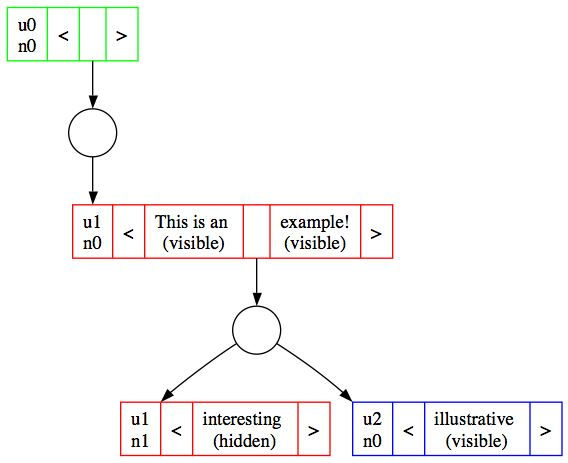
\includegraphics[width=2in]{tree14.jpg}
\caption{Deletion as hiding. Observe that the node $u1/n1$ has the
label "hidden"  beneath its text, whereas the other nodes have "visible".
This indicates that all text in that node is "hidden". \label{fig:tree14}}

\vspace{\baselineskip}%
  \hspace{\fill}\rule{\linewidth}{.7pt}\hspace{\fill}%
\vspace{\baselineskip}%
\end{figure}

\subsection{Inserting into a tree with hidden characters}
Suppose now that user 2 has received all of these edits
and wishes to insert the word ``easy''
into the place where ``interested'' had just been deleted by user 1.
This would result in the following string:
\[
\text{This is an easy illustrative example.}
\]
The point we want to make here is that there are several places that the new node
$X = <^2_0 \text{easy} >^2_0$ could be inserted in the tree
which would place it between "an" and "illustrative" in the string view.
Several possibilities are shown below and their corresponding edit-trees
are snown in Figures \ref{fig:tree14a} and \ref{fig:tree14b}

If the insertion had been done by user 1 rather than user 2, then there
is another option, which would be to modify the edit-tree by appending
"easy" to the text in $u1/n1$ right after the hidden text "interesting".
This is shown in Figure \ref{fig:tree14d}.
\begin{itemize}
\item {\bf leftmost insertion}
The first possibility is to insert the new node directly before the
first character (visible or hidden) after the insertion point. This
is in fact would the current implementation of MSET would select
for this particular example,
but any of these operations could be used.
\[
 <^0_0 <^1_0 
 \text{This is an} 
   <^1_1 <^2_0 \text{easy} >^2_0 \text{\sout{interesting}} >^1_1
  <^3_0 \text{illustrative} >^3_0
  \text{example.} >^1_0 >^0_0
\]
\item {\bf rightmost insertion}
The next is to insert it as far to the right as possible in
the edit-tree.
\[
 <^0_0 \;<^1_0 
 \text{This is an} 
   \;<^1_1 \text{\sout{interesting}} >^1_1\;
  <^3_0 \;<^2_0 \text{easy} >^2_0 \;\text{illustrative} >^3_0\;
  \text{example.} >^1_0\; >^0_0
\]
\item {\bf insertion in a hidden string}
Yet another possibility is to insert it somewhere else (anywhere) in the node $u1/n1$
which contains only hidden text.
\[
 <^0_0 <^1_0 
 \text{This is an} 
   <^1_1 \text{\sout{interesting}} <^2_0 \text{easy} >^2_0>^1_1
  <^3_0 \text{illustrative} >^3_0
  \text{example.} >^1_0 >^0_0
\]
\item {\bf insertion as a child of $u1/n0$}
The final possibility is to insert it as another node at the same level
as $u1/n1$ and $u3/n0$, which would result in
\[
 <^0_0 <^1_0 
 \text{This is an} 
   <^1_1 \text{\sout{interesting}}>^1_1
   <^2_0 \text{easy} >^2_0
   <^3_0 \text{illustrative} >^3_0
 \text{example.} >^1_0 >^0_0
\]
\end{itemize}
These are all the possibly ways in which the edit observed in the string view
could be obtained by a valid edit on the edit-tree.

\subsection{Insertion points depend on the user}
Note, the set of such possible edits depends on which user was doing the
editing. Indeed, 
if the word "easy" had been inserted by user 1 instead of user 2,
then another possiblility
would arise. 

{\bf extension of a hidden node owned by the user}
User 1 could just extend the node $u1/n1$
and not create a new node at all, as shown below and in Figure \ref{fig:tree14d}.
\[
 <^0_0 <^1_0 
 \text{This is an} 
   <^1_1 \text{\sout{interesting}easy}>^1_1
  <^3_0 \text{illustrative} >^3_0
  \text{example.} >^1_0 >^0_0
\]


\begin{figure}[h]
\vspace{\baselineskip}
  \hspace{\fill}\rule{\linewidth}{.7pt}\hspace{\fill}
  \vspace{\baselineskip}

\centering
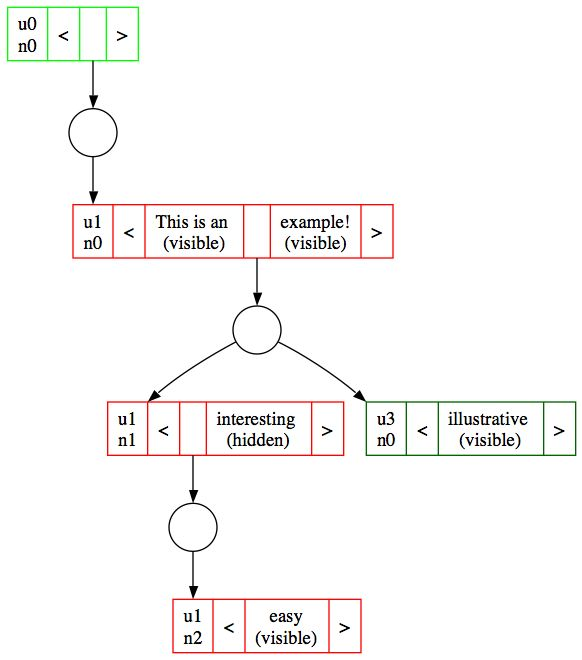
\includegraphics[width=2in]{tree14b.jpg}
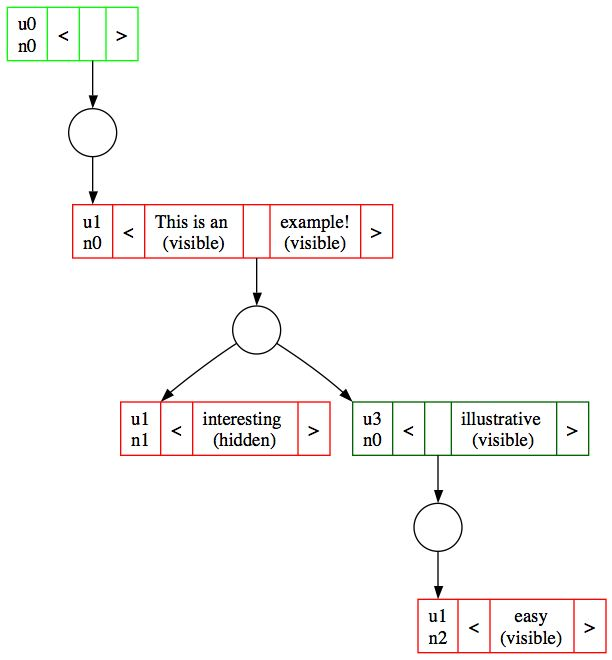
\includegraphics[width=2in]{tree14a.jpg}
\caption{Two ways for user 1 to insert ``easy '' 
between ``an '' and ``illustrative ''. The MSET algorithm
would generate the tree on the left. \label{fig:tree14a}}

\vspace{\baselineskip}%
  \hspace{\fill}\rule{\linewidth}{.7pt}\hspace{\fill}%
\vspace{\baselineskip}%
\end{figure}


\begin{figure}[h]


\centering
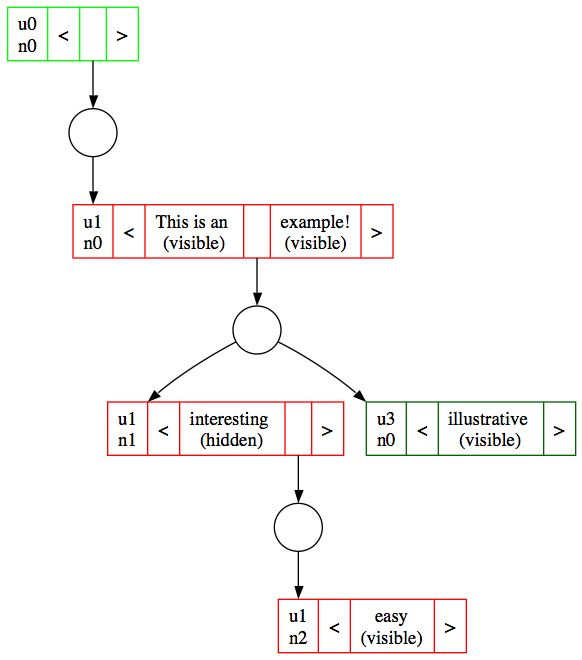
\includegraphics[width=2in]{tree14c.jpg}
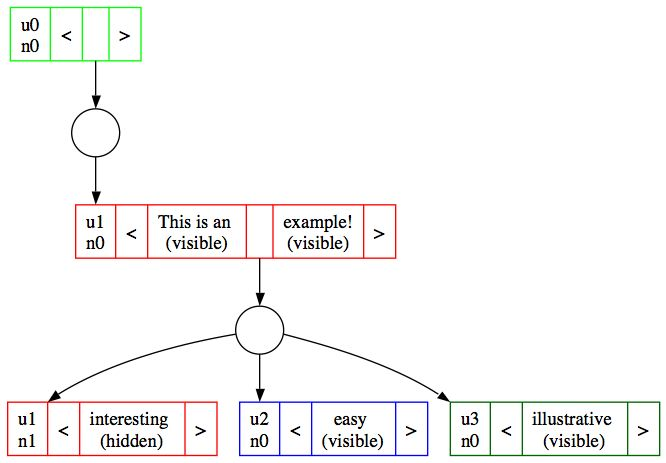
\includegraphics[width=2in]{tree14e.jpg}

\caption{Two more ways for a user to insert ``easy '' 
between ``an '' and ``illustrative ''.\label{fig:tree14b}}


\vspace{\baselineskip}
  \hspace{\fill}\rule{\linewidth}{.7pt}\hspace{\fill}
  \vspace{\baselineskip}

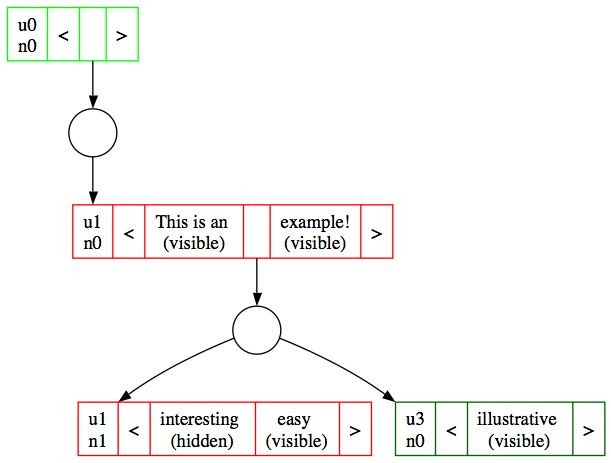
\includegraphics[width=3in]{tree14d.jpg}

\caption{An additional option if the insert was by user 1.
Observe that the text ``easy'' appears with the label ``visible''
in the node $u1/n1$ following the pre-existing hidden text
``interesting'' This is a valid edit operation only if the user
that created the insertion operation is the owner of the node
being extended. In this case, both are $u1$. \label{fig:tree14d}}

\vspace{\baselineskip}%
  \hspace{\fill}\rule{\linewidth}{.7pt}\hspace{\fill}%
\vspace{\baselineskip}%
\end{figure}

Note that we could not insert node $X$ directly before the $<^1_1$ marker
as that would violate the property of edit-trees that all children of a
node attached at the same point must be ordered by their userid and there
must be at most one node for each user. In this case, user 1 would have two
nodes inserted at position 11 of $u1/n0$ which is not allows.

\subsection{General features revealed by the example}
This extended example demonstrates the fundamental ideas behind the MSET
approach. Each user $u_i$ represents the shared document as an edit-tree $T_i$
which has two different views: the standard view $\alpha_i = f(T_i)$ which
is the string of visible characters in $T_i$, and an edit-string view
$\beta_i = g(T_i)$ which contains the hidden characters as well as the
start and end markers for the nodes. The user can insert and delete anywhere
in the standard view, but can only mark characters as "hidden" in the
edit-string view and can only insert at selected places in the edit-string
view. The string operations are converted to edit-tree operations which are
broadcast to all of the peers in the collaborative editing group. Those users
apply the remote operations they receive in any order they choose, provided only
that they wait for the target node of an operation to be created before the'
operation is applied.

We will describe the algorithm in more detail below and we will show that it
can be implemented in such a way that each local and remote edit operation
can be performed in time $O(k\log(N))$ where $k$ is the number of characters
in the operation and $N$ is the size of the edit-string.



\section{The unoptimized distributed model for edit trees}
% Here we describe the model at the level of nodes without worrying about an efficient
% implementation. We can describe the late joining protocol and the central server vs
% distributed server model.

As mentioned in the introduction the MSET model is based on the notion that 
each user maintains an edit tree as the underlying model of the textarea in
which they are editing. In this section, we describe an algorithm for 
collaboratively editing the edit-trees directly. In a later section we will show
how to extend this to an editor of edit-strings as well as strings in
the standard view. Then we'll show how to implement these algorithms
efficiently. In this section, we assume that the users are only interested in editing
the trees directly.

\subsection{Definition of an edit-tree}
We make the following assumptions about the structure of the edit-trees:
\begin{itemize}
\item Each user has a unique ID from some totally ordered set $U$ of userids 
and the nodes of the edit-tree 
are labelled with the userid and an integer which uniquely identifies
that node among all created by that user.
\item Each node contains a sequence of one or more characters.
\item Each character has a boolean visibility property which is set
to false when the character is "deleted". 
\item The nodes can have children nodes.
Each such child is attached at a particular position in the string.
\item Multiple nodes can attach to the same position, but no two nodes that are owned by the 
same user can be attached at the same position. The nodes that are attached at
a given position are ordered by userid. 
\item The root of the tree is owned by the
superuser "u0". This user does not own any other nodes and does not insert any
text into the root node. 
\end{itemize}

\subsection{Valid edit operations on an edit-tree}
We place restrictions on the type of edits that can be performed
on an edit tree. Indeed, there are only three actions a user $u$ can take
when editing their copy of the shared edit tree. We will indicate nodes 
of the edit-tree being edited by
the notation $u/n$ where $u$ is the user who created the node and $n$ is an
integer uniquely identifying this node among all nodes created by the user.

There are three operations a user $u$ can perform on a node and the operations
that can be performed depend on the user.

Let $v/m$ denote the $m$th node created by user $v$.
User $v$ will be able to append characters to the end of $v/m$, so 
we will sometimes futher indicate that node by $(v/m:p)$
where $p>0$ is the number of characters in $v/m$. This allows us to
distinguish between different versions of a single node.

Let $u$ be the user performing one of the following tree tree edit operations
on the target node {\tt v/m:p}.
\begin{itemize}
\item ${\tt treeextend}(v/m:p,\alpha)\;\;\text{if u=v}$ \newline
First, user $u$ can extend the text in the node $v/m$
provided it is the owner (that is $v=u$). It extends the node by appending
some text $\alpha$ to the location $p$ at the end of the node,
Note however, that users can not modify
the text in any node that they do not own and can not change any of the text
once it has been put into the node.
\item ${\tt treeinsert}(v/m:p,q,u/n,\alpha) \;\; \text{if $q\le p$}$
\newline
Second, user $u$ can insert a new node $u/n$ containing a string $\alpha$
at any position $q\le p$ of the node, 
$v/m$ provided
they have not already inserted a node there.
\item ${\tt treehide}(v/m:p,q)  \;\; \text{if $q\le p$}$\newline
Third, user $u$ can set the visibility of a character at position $q < p$
in  $v/m:p$ to false.
When characters are initially added to a node they have visibilty true, but once
set to false, the visibilty must remain false. 
\end{itemize}
For all of these operations, we say that the node $v/m:p$ is the target of the edit operation.

Given these rules we see that a group of distributed users can easily edit a 
shared tree by keeping their own representation of the tree and broadcasting
their edits to their peers. Observe that these edit operations commute in
the following sense. The only place where two user's could have a editing
conflict is when they both want to insert a string of characters at a particular
position $q$ in some node $v/m:p$, but in this case their insertions are always
ordered by userid and this resolves the conflict. No matter which order the
operations are applied the same tree results. This is phrased more formally
in the following lemma:

\begin{lemma}
Let $T$ be any edit-tree and let $\tau_1,\tau_2,\ldots,\tau_n$
be a sequence of valid edit operations on $T$ as described above.
This yields a sequence of edit trees $T_1,\ldots,T_n$. Let 
$\sigma_1,\ldots,\sigma_n$ be any reordering of this sequence of operations
with the property that if $\sigma_i$ has target $v/m:p$, then $v/m:p$ either
exists in $T=T_0$, or $v/m:p$ was created by one of the preceeding $\sigma_i$
which must either be an insert or an extend operation.
Under these assumptions, the corresponding sequence of trees
$S_1,\ldots,S_n$ is well-defined and $S_n=T_n$.
\end{lemma}

\begin{proof}
First, the sequence $S_{i}=\sigma_i(S_{i-1})$ is well-defined because we have
stipulated that the target of each $\sigma_i$ must exist in $S_{i-1}$ so the
operator can be applied. To see that the two resulting trees are equivalent
we simply observe that the extend operations for a node $v/m:p$ must appear
in the same order in the $\sigma_i$ as the $\tau_i$ and since they effect only
the node $v/m$ the node $v/m$ will contain the same string in both $S_n$ and $T_n$.
The insert operations for a given node $v/m$ on the other hand can appear
in any order and their effect will be to add children to positions $q$
of the final node. When multiple insertions attach to the same position, they
will be ordered by user id. Since they are inserted into an ordered list,
the order in which they are inserted doesn't matter.
\end{proof}

\subsection{Distributed editing of edit trees}
In the previous subsection we showed that any valid ordering for a sequence
of tree edit operations will yield the same final result. We can use that
observation to define a distributed algorithm which converges provided only
that a fair network property is assumed.

The model is that we will have a set $G$ of clients $C_1,\ldots,C_n$
all starting with the empty tree. Each client $C_i$ has a unique userid $i$.
and has a local copy $T_i$ of an edit tree,
a history list $H_i$ of edit operations that they have already applied, and
a list $Q_i$ of edit operations that other users have applied but which they
have not yet processed.

We assume that the clients observe the following protocol. 
In particular user $i$ can do the following:
\begin{itemize}
\item Perform a valid operation $\tau$ on their local copy of the tree.
After which they add $\tau$ to $H_i$ and also add $\tau$ to $Q_j$ for
all $j\ne i$.
\item Take an operation $\tau$ from $Q_i$ whose target is in $T_i$, apply
$\tau$ to $T_i$ and add $\tau$ to $H_i$.
\end{itemize}
Note, this model easily allows for late joiners.  Any user $k$ who joins
requests some client $C_j$ to copy its current history list and queue
to $Q_k$. This can be an incremental copy at user $j$'s leisure depending
on the workload.  This may require user $k$ to check each new operation
it receives to make sure that it has not already been received and processed,
but this is not too expensive...

\begin{lemma}
Let $G$ denote a collaborative editing session as described
above and assume that all clients $C_1,\ldots,C_n$ follow the protocol above
for a certain period of time and then stop. Once all queues $Q_i$ have been
emptied and all operations processed, all users will have the same edit
trees, that is $T_1=T_2=\ldots=T_n$.
\end{lemma}

\begin{proof}
This follows easily from the previous lemma where we let $\tau_1,\ldots,\tau_m$
denote the sequence of operations performed by user $1$ and let 
$\sigma_1,\ldots,\sigma_m$ denote the operations performed by user $i$. Then
these are clearly valid rearrangements of each other and by the previous
lemma the resulting trees are the same.
\end{proof}



\section{The unoptimized model for edit trees with a edit-string view}
We are really interested in collaborative editing of strings, not trees, so the
question arises as to how we can convert string edit operations of the user
into tree edit operations on the user's model, and how we can convert tree edit
operations from the user's peers into string edit operations on the user's string,
and how can we efficiently broadcast these edit operations to all other members
of the collaborative edit session.

As a first step, observe that there is a one-to-one correspondence between
edit-strings as defined above and edit-trees, thus our distributed algorithm
for edit-trees provides a distributed algorithm for edit-string where we
assume that the clients $C_i$ each maintain a edit-string $S_i$ and perform valid
edit-string operations on $S_i$. These operations can be transformed directly
into valid tree operations which can be broadcast to the peers above. 

This raises the question of which string edit operations are valid operations,
in the sense that they correspond to the valid tree-edit operations described
in the previous section.  Clearly any non-marker node can be "deleted" by setting
its visibility property to "hidden."  The insertion operations are a little
trickier, but its not hard to show that the following operations are precisely
those which correspond to valid-tree operations. 

We describe the valid edit-string insertion operations as insertions
between two symbols $d_i$ and $d_{i+1}$ in the edit-string, where the $d_i$
is one of the following:
\begin{itemize}
\item  a visible character (denoted $c_i$),
\item a hidden character (also denoted $c_i$),
\item  a start marker $<^v_m$ or
\item an end marker $>^v_m$
\end{itemize}
Let $u$ denote the user performing
the operation and let $n$ be the next available block id for user $u$, so if
the user inserts a new block containing the string $\alpha$, it will be inserted
as $<^u_n \alpha >^u_n$.  Let $c_1$ and $c_2$ denote non-marker characters
which could be either visible or hidden or one of each and let
 $v$ and $w$ be users different from $u$ and each other.

\begin{lemma} Notation as above. The following are precisely the set of valid insert operations, where we indicate the two elements on either side of the insert on the left and the result on the right, together with the condition (if any) that must be satisfied for that insertion to be allowed:
\begin{eqnarray}
c_1\;\;\;\;\; c_2 &\rightarrow& c_1 <^u_n \alpha >^u_n c_2 \label{eq:ins1}\\
c_1\;\; >^w_m &\rightarrow& \left\{ 
  \begin{array}{l l}
      c_1 \alpha >^w_m &  {\rm if}\; u=w  \\
      c_1 <^u_n \alpha >^u_n >^w_m &  {\rm if} \; u \ne w 
  \end{array}  \right . \label{eq:ins2}\\
c_1 \;\;<^w_m &\rightarrow& \left\{ 
\begin{array}{l l}
c_1 <^u_n \alpha >^u_n <^w_m & {\rm if}\; u<w  \\
FAIL & {\rm if} u \ge w \\
\end{array}
\right . \label{eq:ins3}\\
>^v_r \;\;c_2 &\rightarrow& 
 \left\{ 
  \begin{array}{l l}
    >^v_r  <^u_n \alpha >^u_n c_2 & {\rm if} \; v<u \\
    FAIL & if v \ge u \\
  \end{array} \right .\label{eq:ins4}\\
>^v_r \;\;>^w_m &\rightarrow& 
  \left\{
    \begin{array}{l l}
      >^v_r \alpha >^w_m &{\rm if}\; u=w \\
      >^v_r <^u_n \alpha >^u_n >^w_m & {\rm if} \; (v<u)  \&  (v \ne w) \\
     FAIL & {\rm (v > u) \& (v \ne w)}
    \end{array}\right . \label{eq:ins5} \\
>^v_r \;\;<^w_m &\rightarrow & 
\left \{
\begin{array}{l l}
 >^v_r <^u_n \alpha >^u_n <^w_m & {\rm if} \; v<u<w \\
FAIL & {\rm otherwise} 
\end{array} \right . \label{eq:ins6}\\
<^v_r \;\;c_2 &\rightarrow& <^v_r  <^u_n \alpha >^u_n c_2\label{eq:ins7}\\
<^v_r \;\;>^w_m &\rightarrow& 
\left \{
\begin{array}{l l}
<^v_r <^u_n \alpha >^u_n >^w_m & {\rm if} \; v=w=0, r=m=1\\
FAIL & {\rm otherwise} \\
\end{array} \right . \label{eq:ins8}\\
<^v_r \;\;<^w_m &\rightarrow&
\left \{
\begin{array}{l l}
 <^v_r <^u_n \alpha >^u_n <^w_m \;\;\; {\rm if} \; u<w \\
FAIL & {\rm otherwise} \\
\end{array} \right . \label{eq:ins9}
\end{eqnarray}
\end{lemma}

Note that user $u$ can always insert a new node between any two non-marker
characters (Eq. \ref{eq:ins1}), and user $u$ can always insert a string
directly into the end of a node that it owns ($u=w$ cases in Eqs \ref{eq:ins2}, \ref{eq:ins5}).
Also, the only empty node is the root of the tree $<^0_1\;\; >^0_1$ and this
is the only time you have a start marker directly followed by a end marker
(Eq. \ref{eq:ins8}).  The final case to take note of is Eq. \ref{eq:ins7} where
$u$ inserts a string at the between a start-marker and a non-marker characters.
We will come back to these five insertion cases in the next section.

For now, we observe that if a edit-string view only allows the insertions
as shown above for user $u$, then each such insertion corresponds to a valid
edit-tree operation and hence the collaborative editing protocol in the previous
section for edit-trees can be naturally extended to edit-strings. The following
lemma states the convergence property for this distributed algorithm.


\begin{lemma}
Let $G$ denote a set of clients $\{C_1,\ldots,C_n\}$
that are running the collaborative
editing protocol for their local copies of edit-strings $S_i$
starting with empty strings.
Suppose they perform some number of valid
edit operations and then stop editing and process all operations in their queues.
Then, 
we will have $S_1=S_2=\ldots=S_n$.
\end{lemma}



\section{The unoptimized model for edit trees with a standard-string view}

This model is only slightly more complicated than the previous case of
collaborative editing of edit-strings.  In this case, each client maintains
both a standard view of a string (with no deletions and no start/end markers)
and they also maintain the edit-string and edit-tree models in such a way
that these models all agree.

Our first observation is that each character in the standard view corresponds
to a uniquely defined visible non-marker character in the edit-string view. 
Given that observation,
we need to consider the two string operations that a user can perform on a
standard view string and see how we can transform that to an operation on 
the edit-string view.

There are two operations we allow on the standard view:
\begin{itemize}
\item ${\tt insert}(p,\alpha)$ - insert the string $\alpha$ at offset $p$ in the string
\item ${\tt remove}(p,\alpha)$ - remove the substring $\alpha$ begining at offest $p$
which has the effect of changing the attributes of those characters from visible to hidden.
\end{itemize}

If $\gamma$ is a edit-tree and $f(\gamma)$ denotes the standard string view
of that tree, then we want to show that for each string operation $\sigma$
on $f(\gamma)$ there is a corresponding valid operation $\tau$
on the edit-tree, such that 
\[
f(\tau(\gamma)) = \sigma(f(\gamma))
\]
This will allow us to convert string operations into edit-tree operations which
can then be broadcast to all user as in the previous section. There may be many possible $\tau$ operations that satisfy this property (and often there are many), but all we need is the existence of at least one such operation. At this point, we don't worry about the computation complexity of calculating the edit-tree operation corresponding to a string operation, that will be the subject of the next section.

The remove operation is easily transformed into a edit-tree hide operation which 
simply sets the visibility attribute of the corresponding character to ``hidden''.

The insert operation is a bit trickier mainly because, as we have
seen in the example at the beginning of this paper,
a single insert position in
the standard view could correspond to many different insert positions in the 
edit-tree, not all of them legal.


There are four basic insert operations on the string $f(\gamma)$ in the standard view to consider.
\begin{itemize}
\item inserting into an empty string
\item inserting at the beginning of the string
\item inserting at the end of the string
\item inserting somewhere in the middle of the string 
\end{itemize}
The first case is easily handled as it results in the following operation on the 
edit-string $\gamma$:
\[
<^0_0\;>^0_0 \;\; \rightarrow \;\;<^0_0 <^u_0 \alpha >^u_0 >^0_0
\]
The second is a little trickier. We need to find the first non-marker character $d_k$
in the full-edit string and observe that the previous character must be a start
marker $<^v_m$ so we can insert the new node $u/n$ containing $\alpha$ between those
two points, where $n$ is the number of nodes owned by $u$ in $\gamma$ and observe
that inserting a new node 
\[
<^u_n \alpha >^u_n
\]
between a start marker and a non-marker character is always valid.

The third case of inserting at the end of the standard view is similar. One
must find the last non-marker character (visible or hidden) $d_k$ in the
edit-string $\gamma$ and observe that $d_{k+1}$ must be an end marker
$>^v_m$ thus we can insert $u/n$ between $d_k$ and $d_{k+1}$ as a valid
edit-string operation.

The last case is when we are inserting between two characters $c_i$ and $c{_i+1}$
in the standard view $f(\gamma)$. Let $d_j$ denote the visible non-marker
character corresponding to $c_i$ in the edit-string $\gamma$ and let
$d_k$ denote the next non-marker character. So $d_j$ and $d_k$ are non-marker
characters, all the symbols between them are marker symbols, $d_j$ is
visible, and $d_k$ could be visible or hidden. There are three subcases:
\begin{itemize} 
\item $d_{j+1}$ is a non-marker character, i.e. $d_j$ and $d_k$ are adjacent. 
In this case, inserting
the node $u/n$ between them is always valid.
\item $d_{j+1}$ is an end marker $>^v_m$, again in this case inserting $u/n$
between $d_j$ and $d_{j+1}$ will be a valid insert operation.
\item $d_{j+1}$ is a start-marker. In this case all of the symbols between
$d_j$ and $d_k$ must be start markers, so $d_{k-1} = <^v_m$ is a start marker
and inserting between that symbol and the non-marker character that follows
is a valid operation.
\end{itemize}
In each of these three cases, we get a edit-string operation $\tau$ that
corresponds to inserting $\alpha$ between $c_i$ and $c_{i+1}$. The arguments
above have proven the following lemma.


\begin{lemma}
Let $\gamma$ be a edit-tree and let $f(\gamma)$ be its standard string view, then
the algorithm described above constructs a valid edit-tree operation $\tau$
on $\gamma$ for each valid edit operation $\sigma$ on the string $f(\gamma)$, and
we have
\[
\sigma(f(\gamma)) = f(\tau(\gamma))
\]
\end{lemma}


We can now define a
collaborative editing algorithm where the $i$th client presents 
a standard view of a
string $\alpha_i$
to the $i$th user who can then perform arbitrary string
operations on that string.

These string operations $\sigma$ on $\alpha_i$ 
are then transformed into valid edit-tree operations $\tau$
on the underlying edit-tree $T_i$ and these operations are then handled as in the
collaborative edit tree operation. We again have a correctness proof. Moreover, 
this algorithm easily allows one to switch between the two  views: 
the standard string view and the edit-tree view (or more precisely the
edit-string view which is a string representation of the edit-tree).

\begin{theorem}
The full-edit-tree collaborative editing algorithm as described above
is convergent, that is, if all users start with the same tree $T_i=T$ and
all perform a set of editing operations as described above, then after all
editing has stopped and all messages have been received and processed, all clients
will have processed the same number $n$ of edit operations (some local and
some remote) and all will have the same edit tree stored in their local copy
$T_i$.
\end{theorem}


So far we have described a relatively simple collaborative editing algorithm and
proved that it is correct . We have not shown however how
to implement it efficiently. A naive implementation would require time $O(N)$ for
each step, where $N$ is the size of the edit-string. (This would happen
for example if the edit-tree is comb-shaped which would require time $O(N)$
to traverse from the root to the farthest leaf.)

We will show in the 
next section, that this time can be reduced to $O(k\log(N))$ where $k$ is the
size of the operation (i.e. number of characters inserted or deleted) and
$N$ is the size of the edit-string (i.e. the number of characters inserted
and/or deleted by the collaborative users).


\section{Optimizing the model}
% Here we describe the subnode implementation with red-black trees and the initial and
% final subnodes for each node. We prove that the operations are optimally efficient.

We have shown that edit-trees can be used to implement a collaborative editor
which allows the user to immediately apply local edits and which has the convergence
property.  The model as presented in the previous section becomes unacceptably slow as the size of the tree grows.  In this section, we show how to optimize this model by creating a more complex representation which allows
the string to tree and tree to string conversions on edit operations to be computed
in time $O(k\log(N))$ where $N$ is the size of the edit tree and $k$ is the number
of characters in the operation (i.e. number inserted or deleted).

In particular, the MSET algorithm will maintain the edit tree as described above,
but will also maintain an auxiliary data structure $M$ that allows it to rapidly
compute the node position in the edit tree corresponding to an element (i.e. a visible or hidden character or a start or end marker) in any one
of three string views, and vice versa. The three string views are
\begin{itemize}
\item $M.S$: the "standard" list of all visible characters
\item $M.T$: the "tracking changes" list of all visible and hidden characters
\item $M.E$: the "edit-string" list of all edit-string characters which faithfully represents the edit-tree by showing all visible and hidden characters and all markers (both
start markers and end markers)
\end{itemize}
We will show that these three lists can be implemented in such a way as to be able
to calculate the $k$th element of each list (e.g. M.E[k]) in time $O(\log(N))$ where $N$ is the size of the edit-tree.

More precisely, we will describe a new data type, which we call the Monotone Shared Edit Tree datatype which maintains 3 simultaneous representations of a user's edit-session corresponding to the standard, tracking changes, and edit-string views discussed above. This data type allows users to perform two operations locally on their standard view:
\begin{itemize}
\item $insert(k,\alpha)$ - insert string $\alpha$ at offset $k$
\item $delete(k,\alpha)$ - remove the string $\alpha$ which begins at offset $k$
\end{itemize}
These operations are applied converted into edit-tree transforms of the following three types
and are applied locally and also broadcast to all peers in the collaborative edit session:
\begin{itemize}
\item ${\tt treeextend}(v/m:p,\alpha)$ which extends the node by appending
some text $\alpha$ to the location $p$ at the end of the node.
\item ${\tt treeinsert}(v/m:p,q,u/n,\alpha) $ which
 inserts a new node $u/n$ containing a string $\alpha$
at position $q\le p$. 
\item ${\tt treehide}(v/m:p,q)$ which sets
 the visibility of a character at position $q < p$
in  $v/m:p$ to false. 
\end{itemize}
The other users are also editing their local copies and broadcasting these three types of edit-tree transformations to their peers. The MSET data type applies each of these remote transforms to the edit tree as they arrive.

In the rest of this section we will define the MSET data type and prove that each of the local and remote operations can be performed in worst case time $O(\log(N))$



The MSET data type $M$ is implemented by maintaining the three list views using balanced binary trees on the indices so that the element at position $k$ in any of the views can be referenced in $O(\log(N))$ steps.  This is accomplished using a balanced binary tree where each node contains the number of elements in its subtree. Lookup and insertion can be performed in time $(O(\log(N))$.

We will represent each of the characters (visible, hidden, or marker) uniquely as an
element of type Atom.  With this approach, the lists $S$ and $T$ are sublists of $E$.

An Atom element will have the following fields:
\begin{itemize}
\item $nodepos$ this takes values of the form $(u/i/p)$ which specify the position $p$ of the atom in the $ith$ node created by user $u$.
\item $visible$ - this boolean value is true if the character is visible, false otherwise. It is false for the marker symbols and characters are "deleted" by setting this field to false.
\item $character$ - this is the character at that position which is either a character typed in by the user, or is a start marker $<^u_i$ or an end marker $>^u_i$.
\item $node$ - this is a pointer to the particular node in the edit tree containing the character.
\end{itemize}

Each node $N$ in the edit tree will be represented by the following components:
\begin{itemize}
\item $N.user$ which is the user who created this node
\item $N.nodecount$ which is the number of nodes created by the user before this one
\item $N.atom$ which is an arraylist where $N.atom[i]$ will be a link to the $i$th atom in the node, where $i$ is a position consisting either of a non-negative integer or one of the values $startmarker$ or $endmarker$.
\item $N.insertionSet$ where $N.insertionSet[k]$ is a balanced binary tree map $S$ of the nodes inserted at position $k$ in the node, and $S(u)$ gives the node $n$ owned by user $u$ and inserted at that position, if it exists; or gives a pair of nodes $n1,n2$ on either side of the position where a node owned by user $u$ should be inserted. We need this data structure to be able to rapidly process remote insertions with conflicts at the same position in a node. 
\end{itemize}



%We assume that $N$ can be used to find the
%Likewise, we must be able to rapidly compute the inverse functions $g_s(n,o)$, $g_t(n,o), g_e(n,o)$ which give the offset in the specified string ($s,e,n$) corresponding to the specified node $n$ and offset $o$ within that node.
%
%The position of a character in the edit-tree is specified by the node ($n(u,i)$ where $u$ is the unique user id and $i$ is a counter unique for that user) and by the offset $j$ within that node. Recall that for the $i$th node of user $u$,  offset 0 corresponds to the start marker $<^u_i$ and that last position $k+1$ in the node corresponds to the end marker $>^u_i$, assuming there are $k$ characters (visible and hidden) in that node.

%To maintain $M$ one needs to
%explicitly specify information about which node positions are entered in the full
%tree.  We will create node position objects which contain information about 
%which node they are in and in which position (e.g. either an index or, for
%markers, the start or end position). Observe that a {\tt nodepos} is specified
%by $u/n-p$ where $u/n$ is a node and $p$ is the position of a character
%in that node. To be precise, we let $p=0$ denote position of the start marker,
%and $p=i$ for the $i$-th character in the node, and $p=K+1$ for the end merker
%where there are $K$ non-marker characters in the node. The data structure $M$ is
%represented as a doubly linked list of the node positions as they would appear 
%in the full-edit-tree.



%There are two lookup operations:
%\begin{itemize}
%\item {\tt M.lookupNodePos(strpos,view)} - return the node position corresponding
%to the character at the specified string position in the specified view.
%
%\item {\tt M.lookupStrPos(nodepos,view)} - return the string position in the
%specified view of the character at the specified nodepos in the edit-tree.
%\end{itemize}
%where {\tt view} specifies the current view and is either {\tt standard} ($s$),
%{\tt tracking} ($t$) or {\tt edit-tree} ($e$) as described above.
%
%There are also two insertion operations which must be called when
%new characters and/or nodes are added to the edit-tree. 
%These add the newnodepos, directly before or after the character at the specified nodepos in the full-edit-tree view of the edit-tree.
%\begin{itemize}
%
%\item {\tt M.addNodePosAfter(nodepos,newnodepos)}
%
%\item {\tt M.addNodePosBefore(nodepos,newnodepos)}
%
%\end{itemize}
%
%
%Finally, we have an operation which changes the visibility attribute of a node:
%\begin{itemize}
%
%\item {\tt M.hideNode(nodepos)}
%
%\end{itemize}
%which must be called whenever we hide a node $(n(u,i),p)$ in the edit-tree.


%\subsection{Efficient implementation of $M$}
%The data type $M$ can be implemented for each of the three views separately
%by maintaining a balanced binary tree whose leaves are the node positions
%in the current edit tree and where each internal node stores the number
%of characters in the subtree emanating from that node. One can find the
%node position corresponding to a string offset by traversing from the root
%down to a leaf. Likewise, one can find the offset of a node position by traversing
%upward from the corresponding leaf to the root. Hiding a node can be performed
%by traversing from the corresponding leaf to the root and subtracting one
%from each intermediate node for the standard view. Inserting nodes before
%or after a given node requires adding a node and rebalancing. The algorithm
%now depends on which kind of balanced trees are used.
%
%%%% This needs more explanation
%%%%
%Observe that $M$ can be viewed as maintaining three doubly linked lists
%where it takes time $O(\log(N))$ to traverse from one list element to the
%previous or next.
%
%Note that we can compute the edit-string offset $q$ of a character
%$c$ at offset $p$ in the standard-view by
%\begin{verbatim}
%n = M.lookupNodePos(offset,standard)
%q = M.lookupStrPos(n,full-edit-tree)
%\end{verbatim}
%and this takes time $O(\log(N))$

%We also need some data structures to represent the nodes efficiently.
%Each node is represented by 
%\begin{itemize}
%\item an arraylist of attributed characters (visible or hidden or marker)
%\item an arraylist of {\bf insertion sets} for each position in the node. 
%Nothing can be inserted at position 0 as that is before the start marker.
%\end{itemize}
%An arraylist is a data structure that allows one array access to its elements
%and which automatically grows the array when needed.
%
%Each {\bf insertion set} allows one to quickly  insert a new node 
%in the insertion set (i.e. in time $O(\log(N))$)
%and to quickly (i.e. in time $O(\log(N))$ find the node (if any) that appears before and/or
%after the newly inserted node. We can use a binary tree map indexed by
%the userid to implement an insertion set.
%
%When processing remote edit operations, we will need to rapidly lookup
%the node of the edit tree corresponding to a given $u/n$. For this purpose
%we can use a balanced binary tree using the lexicographical ordering on
%node ids $u/n$. This takes time $O(\log(U*N)$ to lookup the node from its
%name, where $U$ is the number of users and $N$ is the total number of insert operations
%applied by all of the users.  
%In practice, for a bounded number of users, 
%we could also use a hash table and get time $O(1)$


\subsection{Local Insertion in MSET}

In this section we show how implement the local insert operation 
\[
insert(k,\alpha)
\]
for user $u$ assuming that it has already created $n$ nodes and that $\alpha$ has length $d$. This will get converted into one of the following two operations:
\begin{itemize}
\item ${\tt treeextend}(v/m:p,\alpha)$ 
\item ${\tt treeinsert}(v/m:p,q,u/n:d,\alpha) $
\end{itemize}
and so we must determine which type of transform is appropriate and to find the node $v/m:p$ and possibly the offset $q$ 
in time $O(\log(N))$.
Once these are calculated, they can be applied in time $O(\log(N))$ by using
a balanced binary tree search to find the node with id $v/m:p$ and the extension
of that node or the insertion of a new node can then be completed in time $O(d)$.

%Note also that the MSET data type, only allows insertion and deletion in the "standard" view. The other two views ("tracking changes" and "edit string") are read only and switching between views can be done in time $O(N\log(N))$ by looking up each of the at most $N$ characters in order in time $O(\log(N))$ for each character.

%The insert position $k$ is either at the beginning or end of the string, or is between
%two consecutive visible characters, $M.S[k-1]$ and $M.S[k]$ but if one shifts to the edit-view, then
%there may be an arbitrarily large sequence of hidden characters between those
%two visible characters. Clearly, any position among the hidden characters
%would correspond to the same position in the standard view. One natural choice would
%be the position immediately after the first character, i.e. before all of the hidden
%characters.  After we make that choice, we can assume that the user is inserting
%a string in the edit-string view.
%
%We will let $N$ denote the size of the edit-string (i.e. the total number of
%hidden and visible characters in the string).


%\subsubsection{Local Insertion}
%Lets consider the case where user $u$ 
%is inserting a string $\alpha$ at position $p$ in the standard string view
We will follow the cases from section ????

Lets look at the simple cases first, that is where we are inserting at the
beginning or the end of the string. 

In the insertion is at the beginning ($k=0$), we need to find the first non-marker (hidden or visible) element $A=M.T[0]$ in the "tracking changes" view which will be at offset 0 in a node $v/m:p$. This takes time $O(\log(N))$.
From $A$ we can lookup the node id $v/m:p$ in constant time so the operation gets transformed into 
$tree_insert(v/m:p,0,u/n:d,\alpha)$
 
This case of inserting at the end is similar, except that we need to find the last element $A$ in the tracking changes view. This can be done in time $O(\log(N))$. From that Atom we can find the
id $v/m:p$ of the node containing $A$ in time $O(1)$ and if $u=v$ then we generate an 
$extend$ operation at position while if $u\ne v$ then we generate an insert at position $p$, the end of the node. 

This leaves the cases involving inserting into position $k$ in the middle of the string.
The first step is to look up the atoms $A_1=M.S[k]$ and $A_2=M.S[k+1]$ on either side of
the insertion point in the standard view and we then calculate the offset $k'$ of $A_1$ and $k''$ of $A_2$ of these atoms in the edit-string view and
the element $A' = M.E[k'+1]$ following $A_1$. This takes
$O(\log(N))$ time. There are three cases to consider.

\subsubsection{Case 1: the element $A'$ in the edit-string is a non-marker character}
In this case, we can lookup the node $v/m:p$ and offset $q$ of $A'$ in constant time and insert the new node containing $\alpha$ between $A$ and $A'$.

\subsubsection{Case 2: the element $A'$ is an end marker for node $v/m:p$}
In this case, if $u=v$ then we can extend the node using $\alpha$ and otherwise
we insert a new node containing $\alpha$ at the end of $v/m:p$.

\subsubsection{Case 3: the element $A'$ is start marker}
In this case, all of the elements between $A_1$ and $A_2$ must be start markers
and so we can insert $\alpha$ right before $A_2$.  So we look up the node id $v/m:p$ of $A_2$ and insert a new node at position $0$.

These arguments show that any insert operation can be converted to an edit tree operation in time $O(\log(N))$.



\subsection{Local deletion in MSET}
Consider now the problem of deleting $k$ characters 
starting at position $p$ of the string.
We will implement this by deleting one character at a time, though this can be
improved (as we will discuss later.) So lets assume that $k=1$. In this case,
we find the node $v/m:p$ and offset $q$ corresponding to the character $c$ to be deleted by looking up $M.S[p]$ in time $O(\log(N))$
and we simply set the visibility flag to "hidden" for that character.

\subsection{Remote extension in MSET}
Lookup node to extend in time $O(\log(N))$
extend in time $O(1)$.

\subsection{Remote insertion in MSET}
Lets now assume we have received a remote insertion operation $\tau$
to insert a new node $v/m$ containing a text string $\alpha$  
at position $p$ 
in the node $u/n$

Our first step is to lookup the node $N$ with id $u/n$ in time $O(\log(N))$
and then to access the insertionSet $S=N.insertionSet[p]$ at offset $p$
and then to create a new node $N'$ with id $u/n$ containing $\alpha$.
This insertion set is between two elements $A$ and $A'$ of the edit-string.
There are a few cases.

If $S$ is empty, then we simply insert $N'$ into $S$ and insert the elements
corresponding to $\alpha$ into the appropriate positions in $M.S$, $M.T$, and $M.E$. This can all be done in time $O(\log(N))$.

If $S$ is not empty, then it holds a sequence of nodes by different users and none of those nodes are owned by $u$.  Since it is a balanced tree we can lookup the position where $N'$ needs to be inserted in time $O(\log(N))$. There are three
cases. First, if $N'$ needs to be inserted at the beginning of $S$, then 
it will be inserted directly after $A$. Likewise, if $N'$ needs to be inserted at the
end of $S$, then it will be inserted directly before $A'$. 

The only remaining case, is that $N'$ must be inserted between consecutive two nodes $N_1$
and $N_2$ in S. We then lookup the end position element $B$ of $N_1$ and insert $N'$ directly after $B$.


\subsubsection{Remote hiding in MSET}
The problem of processing a remote operation $\tau$ to hide 
a character at position $q$ in node $v/m:p$ is easier.

We lookup the node with id $v/m:p$ in time $O(\log(N))$ and
then we find the element at position $q$ in the node
and set the attribute to $hidden$ in time $O(1)$.

\subsection{Main theorem}
We have therefore proved 

\begin{theorem}
The MSET data type processes each of the two local operations (insert and delete) and
the three remote operations (treeextend, treeinsert, treehide) in time $O(k\log(N))$ where $N$ is the size of the edit-tree before the operation is performed and $k$ is the size of the string $\alpha$.
\end{theorem}

\section{Extensions}
???


%%%%  Work getting parts of the rest of this into the main article
%\newpage
%\section{Details of a Pratical M}
%In practice, we don't use node positions of size 1 but rather use subnodes
%of size 1 or more that consist of sequences of characters that all share the
%same attribute (e.g. hidden or visible). This complicates the algorithms
%as deletion requires one to split subnodes which are then reinserted into
%the data structure $M$, but it greatly decreases the speed of the algorithm
%(not asymptotically of course). Moreover, we don't introduce explicit
%start or end marker nodes of size zero unless they are needed, which only
%occurs if there is an insertion at the beginning or at the end of a node.
%
%Also, discuss algorithms for preferring extensions rather than
%inserts where possible.
%
%%% KGG needs to change data references to characters to maintain consistency
%
%\subsection{Introducing Subnodes}
%$Subnode$: A reference to a segment of an MSET node's sequence of characters that
%share the same set of attributes and does $not$ have any insertions.
%
%Bold Assertion: We can't minimize node creation by merging node data (e.g.
%creating strings from characters) without introducing subnodes. To do so would
%restrict the use of attributes.
%%lookup times to degrade to O(N) vs O(log(N)).
%
%%% I'm not sure that our auxiliary data structure $M$ is to be viewed as three
%%% doubly linked list as described in section 6.1 Efficient implementation of M
%%% but rather as described in this section as one large doubly linked list of 
%%% subnodes and N=(number of nodes) smaller linked list.
%
%Thus far we have discussed the MSET data structure as a tree of nodes containing
%an arraylist of attributed characters and an arraylist of insertion positions.
%Now we are going to introduce subnodes that place the markup
%of raw MSET data on a separate plane, but more importantly, 
%enables the grouping of sequences of characters with identical attributes.
%That is, the raw MSET data (full string view)
%is still stored in MSET nodes as it did before, but now, attributes are stored
%in a linked list of subnodes for optimum maintenance. This also enables faster
%seek times at the expense of extra meta data.
%
%%Another significant reason for including subnodes is to optimize the MSET node
%%space complexity by introducing node extensions. 
%
%$Node Extension$: Append newly inserted data $k$ at the end of an existing node's
%data $N(c)$ instead of creating a new node when the following rules are upheld:
%
%%% rule 1) is greatly simplified here because it is not handling full view
%%% and standard view differences. Mainly, the most frequent case of hitting the
%%% backspace key as we type prevents real extensions unless we check for it.
%\begin{verbatim}
%  1) The new data is being inserted at the end of a node.
%  2) Both the new insertion and the node that is to be extended is
%     owned by the same user.
%\end{verbatim}
%
%These rules are required to maintain MSET's convergence mechanism, uniquely
%ordered and identifiable edits. With insertions being identified by u/n/p,
%allowing extensions of any other form would corrupt the MSET.
%
%
%
%\subsection{Balanced Lookup Trees}
%The core principle of an MSET is that all edits are permanent, one directional,
%monotone. This principle is to be extended to attributes as well. To do so more
%clearly we introduce balanced subnode trees that are provide the means for
%fast conversions between node positions and string offsets (M.lookupNodePos, 
%M.lookupStrPos) and also maintains the attribute set of raw MSET data.
%
%As described before, we are just balancing an indexed MSET based inserts and
%attributed node segments to achieve O(log(N)) lookup complexity when going back
%and forth between node view and string view. The idea is to have all the subnodes
%make up the leaves of the balanced binary tree. Thus each parent node would
%pivot on the sum of its children sizes as depicted in \label{fig:rbtree14e}.
%
%\begin{figure}
%\centering
%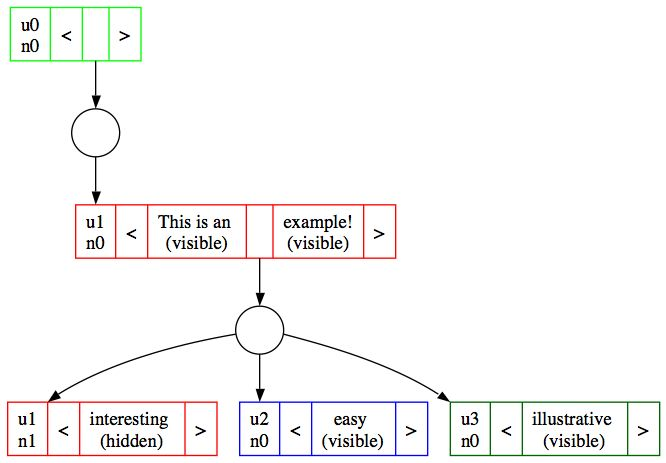
\includegraphics[width=2.4in]{tree14e.jpg}
%%\includegraphics[width=2.4in]{tree14e-rb.png}
%
%\caption{Natural Node View -VS- Balanced Binary Subnode View.\label{fig:rbtree14e}}
%
%\vspace{\baselineskip}
%  \hspace{\fill}\rule{\linewidth}{.7pt}\hspace{\fill}
%  \vspace{\baselineskip}
%\end{figure}
%
%A global balanced tree $GT$ sits a top a linked list of all subnodes and each
%MSET node has a local balanced tree $LT$ that sits a top a linked list of its
%subnodes. 
%
%
%\newpage
%\section{Extensions}
%\subsection{Allowing more general attributes}
%One simple extension to this model allows it to support general text attributes
%(e.g. font-style, text-color, etc.) which can be changed multiple times by
%the users while preserving the convergence property.
%
%The key idea is to associate with each character both an attribute set and a
%priority value. The priority value consists of a positive integer $k$ and a userid $u$
%indicating the author of the last change and the priority of that change. 
%When a user $u$ changes an attribute, the generate a tree edit operation which
%increments the priority $k$ and sets the author to $u$. When a user receives
%a remote attribute change operation with priority $(k',u')$ it compares that
%priority with the current priority $(k,u)$ and only applies the attribute
%change if $(k',u') > (k,u)$, that is if $(k'>k) \vee (k=k')\wedge(u'>u)$.
%Note that unless we use an unbounded representation (e.g. java.math.BigInteger)
%for the priority $k$
%that there will be a maximum priority $k_max$ after which no additional
%changes to the attribute set will be allowed. This is probably not a practical
%problem if one uses at least 16 bits for the priority.
%
%This extension works well with the subnode optimization as one can associate
%an attribute to an entire subnode and hence change the attributes of the text
%in a subnode in time $O(1)$
%
%
%\subsection{Late Joining}
%Late joining can be implemented by allowing a late joiner to ask another
%user to send its history and queue to the late joiner.  The late joiner
%keeps track of which nodes it has received from each user and can tell
%when it is up to date. This assumes that the users generate node id's
%sequentially.  To optimize this we can structure the history mechanism
%as ordered list of users, and for each user a vector of edit operations
%and a vector of "holes" which are operations that have been generated but
%have not yet been received.  In addition, each node it will contain an
%ordered list of extension operations.
%
%\subsection{Adding backchannel communication}
%We have found it useful to increase awareness by adding video, audio, or
%text-based communication to the editing session. This is not an algorithmic
%extension to the editor, but in practice most user's do have the ability to
%add an audio or visual connection.  For large groups that are not collocated,
%a shared text-based chat window would also work, possibly with speech generation
%to keep the visual space free.
%
%\subsection{Managing the queues of incoming and outgoing edit operations}
%The MSET model can easily accommodate the introduction of queues of incoming
%and outgoing tree-edit operations and we have found it helpful to allow the
%user to turn on an off the queueing of incoming and/or outgoing edit operations.
%Queueing the incoming edit operations
%is similar to locking a document in that a user's edit session is not
%interrupted by remote edit operations but remote users are able to continue 
%editing and can even edit the user's text as it is being generated. This
%is particularly useful when the user is performing a repeating macro on
%the edit window (e.g. applying some emacs-macro to every line of a file).
%It is also useful when entering an "undo" session as we describe in the next subsection.
%
%Queueing both incoming and outgoing operations is helpful if the user wants to
%work on a part of the document and doesn't want any other user to be able to
%edit the section until it is complete.  This is helpful for example, when
%co-editing a Java program if the user is refactoring a procedure. Other users
%can continue to edit and compile the code without these changes being visible
%until they are complete.
%
%Disconnection from the network can be handled transparently by turning on the
%queueing of incoming and outgoing edit-operations. When the network is rejoined
%the user perform a late joining request to another user (ideally a high bandwidth)
%user, where that user sends its history and queues to the reconnecting user
%in reverse order (i.e. most recent first). The reconnecting user filters out
%those operations that have already been processed (and are in the 
%node lookup table)
%
%\subsection{Undo}
%
%It is a good idea to enter an "undo" mode in which all incoming edit operations
%are queued while the undo process is active as this will allow the user to
%revert the system to the state they want before continuing.
%
%\subsubsection{Global Undo}
%The simplest form of "undo" which reverses the most recent non-undo edit operation
%is easy to implement.  One keeps a history of the string-based edit operations
%as with a usual text-editor and then issues the reverse operations as local
%operations.  This will not actually revert the underlying edit-tree to a previous
%form, rather it will mark nodes created initially by an insert as having
%"hidden" characters, and it will generate a new insert operation, to "undo"
%a "delete" operation. The usual approach of combining insertions of characters
%into a single string for the purpose of undo can also be performed.  
%
%
%\subsubsection{Selective undo}
%One can also undo operations created by a single user (usually the user
%him/herself). This can be done by walking through the history in reverse
%order and converting the tree-edit operations performed by that user into
%reverse operation that would have the effect of undoing the operation
%at the string level.  That is, an insert operation gets converted into a
%"hide" operation, and vice-versa. There is some ambiguity about where to
%perform the insert corresponding to a hide, but it doesn't affect the 
%correctness or complexity of the algorithm, so any choice will do.
%
%One could also selectively undo all operations except those by a particular
%user, or selectively undo all operations by some set of users. This generality
%is easily obtained by generating undo operations at the edit-tree level.
%
%\subsection{Enhancing the view to support awareness features}
%We have found it helpful to modify the standard string view in a few
%ways to help increase the awareness of what other users are doing. 
%
%\subsubsection{Visual cues for user positions}
%The simplest and most helpful extension is to associate to each user a
%color (which they can change in their preference pane) and to indicate
%the each user's location by highlighting the 10-20 characters to the left
%of that user's current location using that user's color.  One can use two
%different notions of a user's location:
%\begin{itemize}
%\item the location of their last edit operation, or
%\item the current location of their cursor
%\end{itemize}
%The key point here is that we indicate the user's location by specifying
%the position of a character in the edit-tree and broadcasting this to all
%of the peers. Thus, even if user's have completely different edit-trees at
%some point, the user positions are well-defined.  One interesting phenomenon
%howeveer is that user $u1$ could be editing a node $N$ that has not yet
%been created by user $u2$, in this case user $u1$'s location will be off-screen
%until the operation that creates node $N$ in $u2$'s edit-tree is executed.
%
%\subsubsection{Tracking users}
%Another useful feature is to allow the user $u$ to specify an other user $u'$ to
%be tracked. Whenever the user $u'$ changes location, the view of user $u$
%scrolls to keep those edits in view.
%
%\subsection{Easing the restrictions on the ordering of edit-operations}
%Another easy extension is to introduce another text attribute, 
%"undefined", in addition to the "visible" and "hidden" attributes. Characters
%in the node would start off with the "undefined" attribute, which could be
%changed to "visible" and then to "hidden".  With this model, extension
%operations could be performed out of order by setting the attribute of
%all characters from the end of a node to the beginning of the extension to
%be "undefined".
%
%Another enhancement is to allow the system to combine edit operations
%in the cache. More precisely, we can view the client as building a forest
%of edit-trees. So, when an edit-operation is received whose target has
%not yet been received, the system can create a virtual target node
%with all characters undefined and start applying the edit operations to
%that node, even though it has not yet been received. When the edit-operation
%that creates that node is finally received, the node can be added directly
%to the edit-tree in one step.  One still has to merge the MSET structures
%for the main tree and this subtree, this can be done in time $O(\log(N))$
%because the MSET-structure for the subtree can be merged into the MSET
%structure for the main tree in time $O(\log(N))$.
%
%HMMMM.  WE NEED A PROOF FOR THIS. I HAVE A GENERAL IDEA OF HOW IT WOULD WORK
%BUT IT DEPENDS ON THE PARTICULAR IMPLEMENTATION OF THE MSET THAT WE USE, E.G. 
%RED-BLACK, 2-3-TREE, ETC.
%
%The view for this more general approach would include the main tree, but would also
%allow the user to view the other trees in the forest
%
%\subsubsection{Pulling versus Pushing}
%Another extension is to allow clients to request the sequence of ancestor nodes
%for a particular node. This would allow user's to merge the trees in the forest
%into a single tree, although many of the nodes connecting the main tree to the
%subtree will be "virtual" nodes consisting entirely of "undefined" characters.
%If the ancestor sequence is sent one node at a time, the receiving user can
%signal the sender to stop once it has reached ancestors that are already in the
%receivers tree. A user could also ask a client to sent the sequence of edit
%operations needed to reconstruct the path from the given node to the root.
%This would require higher bandwidth but would also produce more context for the
%subtree.
%
%
%\newpage
%\section{Analysis and Benchmarks}
%
%Analyze the parameter that determine how many users can 
%simultaneously edit a document at what speed.
%
%Validate the analysis with benchmarking experiments.
%
%Here we present the benchmarks that show the performance curves with varying numbers
%of users.  Show KGG benchmarks that demonstrate O(log(N)) performance
%even as the number of users and the number of edits becomes quite
%large.
%
%
%\newpage
%\section{Implementation}
%Here we describe the implementation for JEdit, NetBeans, and the Applet and discuss
%the general approach to collaboratizing a textarea.
%
%
%Describe input and output queues and how the user can store
%outgoing edits in an output queue until reconnecting.
%
%Discuss the preference given to local operations, so that
%the system always looks for a local operation after performing
%each single (and relatively small) remote operation. This
%guarantees that the user can have a responsive system at the
%cost of remote edits lagging a bit.
%
%Discuss the history replay mechanism including forward and
%backward playing.
%
%Cite the 2009 conference paper ...
%
%\newpage
%\section{Applications}
%Here we describe the ways in which we have used CollabEd in the classroom and for
%research.
%
%Group coding (writing a large Java class quickly together or
%creating an HTML page quickly together watching each other
%to learn by doing and watching).
%
%Group debugging - asking users to find errors and correct them
%while we debug together.
%
%Online TAing - using an audio or video link with collabed to
%jointly debug a program.
%
%Grading the process - viewing the replay to better understand
%the problems faced and solved (or not) by a student.
%
%Grading group assignments - viewing the replay to see how the
%students collaborated to complete the program.
%
%Cite our earlier work....
%
%\newpage
%\section{Related Work}
%Here we give an overview of related work both academic and commercial.
%
%\newpage
%\section{Future work}
%Javascript-based clients.  Integration with subversion/cvs/etc.
%Full implementation of attributes. More robust networking --
%handling dropped connections. Multi-file sharing and replay.
%
%Another interesting and challenging problem is to combine MSET with
%operational transformation to handle cut/paste operations more naturally.
%The idea would be to define cut/paste as a tree operation which removes
%a set of subtrees from the tree and creates a new node $N$ where all of
%these subtrees are then reattached. The goal would be assume that there

\bibliographystyle{abbrv}

%is a central server to serialize all of these cut/paste operations (but
%not necessarily the other operations) and then to define an operation
%transformer which will allow multiple users to converge on the same
%edit tree.  The interesting approach here is that the operational transforms
%will be on edit trees rather than on strings.  The benefit to this approach
%is that the edit-tree structure of a cut/pasted section of the document
%will be preserved by the cut/paste operation and the space will not grow
%as rapidly. 


\bibliography{collabed}

%\appendix
%\section{Proofs}
%I think we claimed that we would put some things in the appendix!
\end{document}


%%% Local Variables: 
%%% mode: latex
%%% TeX-master: t
%%% End: 
